\section{Simulations}\graphicspath{{../SimpleSim/}}
In this section, we will focus on two different systems under continuous measurement of their environment. The first system is a qubit (two-levels quantum system), while the second system is a harmonic oscillator (infinite levels). 

Before looking at the diverse simulations, we want to explain the conversion into dimensionless variables we will use for our simulations. By considering the Lindblad master equation, Eq.~(\ref{eq:LindbladME}), we can introduce a dimensionless time $\tau=kt$ such that this equation rewrites as
\begin{equation}
    \frac{\mathrm{d}\rho(t)}{\mathrm{d}\tau} = -\frac{i}{k}\qty[H_S,\rho(t)] + \mathfrak{D}[c]\rho(t). 
\end{equation}
In any of the following cases (simulating a qubit or a harmonic oscillator), the Hamiltonian $H_S$ is proportional to the natural frequency of the system denoted as $\omega_0$. Hence, the first term of the Lindblad master equation yields the dimensionless frequency $\Omega=\frac{\omega_0}{k}$. To respect the weak-coupling condition, it must verify $\Omega\gg 1$, so, in the simulation we chose to set it to $\Omega=10$. We know from OQS theory that after some oscillations, the system reaches the stationary state. Thus, our simulations will span over $\tau\in\qty[0,10]$ to be close enough to the stationary state at the end. This reasoning stands for SME simulations because we know that the average over every possible trajectories gives back the Lindblad unconditional evolution. We precise that the environments of the following systems are always at the zero-temperature limit, i.e., we consider the vacuum state of the environmental oscillator at each time $\ketbra{0}_t$. 

\subsection{The qubit under photo-detection of its environment}
The simulation of a qubit under photo-detection of its environment is realized by implementing the Monte Carlo simulation method into \verb|Julia|. The package \verb|QuantumToolbox.jl| has a dedicated function called \verb|mcsolve| which does it fine. This function requires in particular to specify the Hamiltonian of the system $S$, the initial state (as a vector or a density operator), the number of trajectories to simulate (in order to average over all trajectories) and the operators to apply. 

\begin{figure}[h]
    \centering
    \begin{subfigure}[t]{0.6\textwidth}
        \centering
        
\includegraphics[width=\textwidth]{MCQ/Pop_10000.pdf}
        \caption{The evolution of the excited population of the qubit with respect to dimensionless time $\tau$ compared to the unconditional evolution of the excited population.}
        \label{fig:MCQpop}
    \end{subfigure}
    \\
    \begin{subfigure}[t]{0.58\textwidth}
        \centering
        
\includegraphics[width=\textwidth]{MCQ/histo.pdf}
        \caption{The histogram of simulation jump times $T$ of every simulations compared to the analytical Lindblad PDF.}
        \label{fig:MCQhist}
    \end{subfigure}
    
    \caption{Results obtained from the Monte Carlo simulation of a qubit under continuous photo-detection of its environment. }
    \label{fig:MCQglobale}
\end{figure}

To work with the qubit, we briefly detail the notations and operators used in the description of two-level systems. Firstly, the eigenstates of the Hilbert space $\mathcal{H}_S$ are denoted as $\ket{e}=\mqty(1 \\ 0)$ and $\ket{g}=\mqty(0 \\ 1)$, where $e$ is the excited state and $g$ is the ground state of the qubit. Secondly, the three Pauli matrices that form (together with the identity $\mathbb{I}$) an eigenbasis of $\mathcal{H}_S$ are denoted as
\begin{multline}
    \sigma_x = \ketbra{e}{g}+\ketbra{g}{e}=\mqty(0 & 1 \\ 1 & 0),\quad \sigma_y=-i\qty(\ketbra{e}{g}-\ketbra{g}{e})=\mqty(0 & -i \\ i & 0),\\ \sigma_z=\ketbra{e}-\ketbra{g}=\mqty(1 & 0 \\ 0 & -1).
\end{multline}
We will also use the ladder operators
\begin{equation}
    \sigma_- = \ketbra{g}{e}=\mqty(0 & 0 \\ 1 & 0),\quad \sigma_+ = \ketbra{e}{g}=\mqty(0 & 1 \\ 0 & 0),
\end{equation}
which act respectively as a lowering and a raising operator, inducing transitions from the excited to the ground state and vice-versa. Notice that in a two-levels system, the density matrix is simply
\begin{equation}
    \rho = \mqty(\rho_{ee} & \rho_{eg} \\ \rho_{ge} & \rho_{gg}),
\end{equation}
where $\rho_{ee}$ and $\rho_{gg}$ are respectively the excited and ground populations, and where $\rho_{eg}$ and $\rho_{ge}$ are the correlations. Notice that the definition of a density matrix, see Section~\ref{sec:purity}, implies that $\rho_{ee}+\rho_{gg}=1$, that $\rho_{ge}=\rho_{eg}^*$, and that $\rho_{ee}\rho_{gg}\geq \abs{\rho_{eg}}^2$ in particular.


In the case of the qubit, the no-jump evolution Eq~(\ref{eq:MC}) becomes
\begin{equation}
    \dert{}\ket{\tilde{\psi}_0(t)} = -\qty(\frac{k}{2}\sigma_+ \sigma_- + i\frac{\omega_0}{2}\sigma_z)\ket{\tilde{\psi}_0(t)},
\end{equation}
where $H_S = \frac{\omega_0}{2}\sigma_z$. We can enjoy the transformation of units $kt=\tau$ in order to work with a dimensionless equation, giving
\begin{equation}\label{eq:MCphotodet}
    \frac{d}{\mathrm{d}\tau}\ket{\tilde{\psi}_0(\tau)} = -\qty(\frac{\sigma_+ \sigma_-}{2} + i\frac{\Omega\sigma_z}{2})\ket{\tilde{\psi}_0(\tau)}.
\end{equation}
In anticipation of the simulation, we have seen theoretically in Section~\ref{sec:photodet} that the key quantity available to an experimentalist is the set of photo-detection outcomes $\qty{\mathrm{d}N_t}_t$. The stochastic expectation value of this random variable as been shown to be $\mathbb{E}\qty[\mathrm{d}N_t]=k\expval{c^\dagger c}_t \dt = \rho_{ee}^{(c)}(\tau)\mathrm{d}\tau$, where we denoted the conditional property of this state as $(c)$ for convenience. This average is only stochastic on a single trajectory and we can average over every trajectories to find that $\mathbb{E}_\mathrm{trajs}\qty[\mathrm{d}N_\tau]=\rho_ee(\tau) \mathrm{d}\tau$, where the state is now unconditional. This property is used in the Figure~\ref{fig:MCQhist} to build the so-called analytical Probability Density Function (PDF) from the Lindblad evolution. Indeed, very generally from the OQS theory, one can show that $\rho_{ee}(\tau)=\rho_{ee}(0)e^{-\tau}$~\cite{Breuer}. Therefore by normalizing over the simulation period so that the area under the curve is exactly 1, we find that
\begin{equation}\label{eq:PDF}
    \mathrm{PDF}(\tau) = \frac{e^{-\tau}}{1-e^{-\tau_\mathrm{max}}}.
\end{equation}
This PDF is actually independent of the system choice and will be the same for the harmonic oscillator. This is straightforward to show when replacing the generic $c$ operator by the annihilation operator $a$, and by knowing that $\expval{\hat{n}(\tau)}=\expval{a^\dagger a}(\tau)=\expval{n(0)}e^{-\tau}$~\cite{Breuer}.

The average excited population of every simulated trajectories is compared to the unconditional evolution of the excited population in Figure~\ref{fig:MCQpop}. We have simulated 10,000 trajectories to obtain this graph within the \verb|MCQubit.jl| program (all the programs are available on the GitHub repository {\color{red} LIEN}). In this program, we chose to set the initial state as $\ket{\psi(\tau=0)}=\frac{\ket{e}+\ket{g}}{\sqrt{2}}$, and we can observe that the excited population is indeed 0.5 at the beginning on Figure~\ref{fig:MCQpop}. As expected, the average of the 10,000 trajectories follows the unconditional trajectory. The error inset plot in Figure~\ref{fig:MCQpop} is showing that the difference between these two curves is small enough to consider the result valid. We expect the difference to decrease as the number of trajectory increases. Ideally, we should find exactly the same curves as the number of trajectory tends to infinity. 

Moreover, some single trajectories are plotted on this figure to show their behavior. Theoretically, it is possible that a trajectory never jumps because of the superposition of states initially set. Indeed, if the random number $R$ picked is very small, the system might have time to purify to the ground state before the norm diminishes enough. Specifically, we know that SMes conserve the purity of states and we can observe that the final excited population is 0, meaning that the final state is $\ket{g}$. Hence, the norm is 1 at the end and obviously cannot be smaller than $R$. This reasoning seems to imply a competition between the Lindblad purification of the state and the ability to be measured by the photo-detector.

Furthermore, the curve labeled ``$\rho_{ee}(\tau)$ no-jump (analytical)'' is the evolution of the state without never jumping. To reach the analytical expression of this evolution, we simply have to solve Eq.~(\ref{eq:MCphotodet}). For a generic superposition $\ket{\psi(\tau)}=\alpha\ket{e}+\beta\ket{g}$ with previous units (non-dimensionless), we find
\begin{equation}
    \ket{\tilde{\psi}_0(t)} = \alpha e^{-i\frac{\omega_0}{2}(t-t_0)}e^{-\frac{k}{2}(t-t_0)}\ket{e} + \beta e^{i\frac{\omega_0}{2}(t-t_0)}\ket{g}.
\end{equation}
We can then calculate the square of the state's norm in order to obtain the expression of the mean excited population within the no-jump evolution. We easily find that
\begin{multline}
    \braket{\tilde{\psi}_0(t)} = \abs{\alpha}^2e^{-k(t-t_0)}+\abs{\beta}^2, \text{ so that}\\
    \abs{\braket{e}{{\psi_0(t)}}}^2 = \frac{1}{1+\abs{\beta}^2/\abs{\alpha}^2 e^{k(t-t_0)}}.
\end{multline}
Therefore in our case ($\alpha=\beta=\sqrt{2}$), we have that the dimensionless no-jump evolution is given by
\begin{equation}
    \rho_{ee}^\mathrm{no-jump}(\tau) = \frac{1}{1+e^\tau},
\end{equation}
with the initial condition $\rho_{ee}^\mathrm{no-jump}(0)=\frac{1}{2}$ as expected.

\subsection{The harmonic oscillator under photo-detection of its environment}

This simulation is embedded within the \verb|MCHarm.jl| program with the same function \verb|mcsolve|, as in the last subsection. The initial state is $\ket{\psi(0)}=\ket{\alpha_0}$, where $\alpha_0$=2. This state is a coherent state~\cite{Barnett}, we define it using the Fock states $\qty{n}_{n\in\mathbb{N}}$ as
\begin{equation}\label{eq:coherentfock}
    \ket{\alpha_0} = e^{-\frac{\abs{\alpha_0}^2}{2}}\sum_{n=0}^{+\infty} \frac{\alpha_0^n}{\sqrt{n!}}\ket{n}.
\end{equation}
A key property of this kind of state is in particular that $a\ket{\alpha_0}=\alpha_0\ket{\alpha_0}$, where $a$ is the annihilation operator of the system. Another property is that $\expval{\hat{n}}{\alpha_0} = \abs{\alpha_0}^2$, which is thus the initial mean population of the system. The Hamiltonian of the system is now $H_S = \omega_0 a^\dagger a$, and the no-jump evolution followed by the Monte Carlo process is
\begin{equation}\label{eq:MCharmUNITS}
    \dert{}\ket{\tilde{\psi}_0(t)} = -\qty(\frac{k}{2}a^\dagger a + i\omega_0 a^\dagger a) \ket{\tilde{\psi}_0(t)}.
\end{equation}
In terms of the dimensionless system ($kt=\tau$), this equation becomes
\begin{equation}\label{eq:MCharm}
    \frac{\mathrm{d}}{\mathrm{d}\tau}\ket{\tilde{\psi}_0(\tau)} = -\qty(\frac{1}{2}+i\Omega)a^\dagger a \ket{\tilde{\psi}_0(\tau)}.
\end{equation}
As explained in the last subsection, the PDF in Figure~\ref{fig:MCHhist} is the same as in the case of a qubit, see Eq.~(\ref{eq:PDF}). Therefore, this figure is very similar to the Figure~\ref{fig:MCQpop} as expected. Indeed, the average over all trajectories of the jump times must give the unconditional PDF (which is thus the same for both systems).

The unconditional mean population is given by 
\begin{equation}\label{eq:uncondMCH}
    \expval{\hat{n}(\tau)}=\expval{\hat{n}(0)}e^{-\tau} = \abs{\alpha_0}^2 e^{-\tau}.
\end{equation}
This evolution is represented by the dash-curve labeled by ``$\expval{\hat{n}(\tau)}$ (analytical)'' in Figure~\ref{fig:MCHpop}. We observe that the initial mean population is indeed 4 since $\alpha_0=2$ and because of the last equation. To obtain the simulation curve, we averaged 10,000 trajectories and we see that, as expected, the average evolution curve superposes with the unconditional evolution. However, compared to the qubit case, we see that the errors (present in the inset of Figure~\ref{fig:MCHpop}) are way more small (around $10^{-6}$ order of magnitude compared to $10^{-3}$ at worst). To have a hint on why the error is so low in this case, we might want to calculate the no-jump mean population evolution.



By solving Eq.~(\ref{eq:MCharmUNITS}), we find
\begin{equation}
    \ket{\tilde{\psi}_0(t)} = e^{-i\omega_0a^\dagger a (t-t_0)}e^{-\frac{ka^\dagger a}{2} (t-t_0)}\ket{\alpha_0},
\end{equation}
which will be used t\begin{figure}[tb]
    \centering
    \begin{subfigure}[t]{0.6\textwidth}
        \centering
        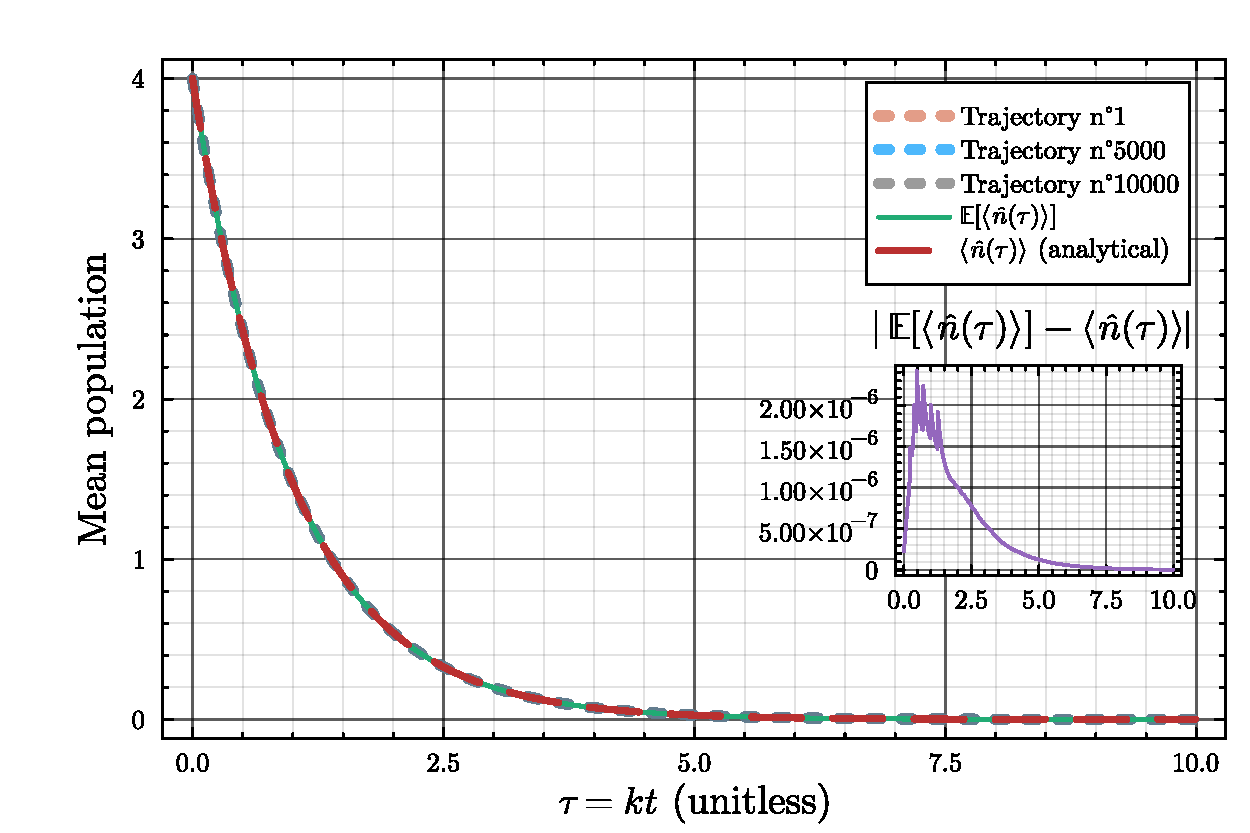
\includegraphics[width=\textwidth]{MCH/Pop_10000.pdf}
        \caption{The evolution of the mean population of the harmonic oscillator with respect to dimensionless time $\tau$ compared to the unconditional evolution of the mean population.}
        \label{fig:MCHpop}
    \end{subfigure}
    \\
    \begin{subfigure}[t]{0.58\textwidth}
        \centering
        
\includegraphics[width=\textwidth]{MCQ/histo.pdf}
        \caption{The histogram of simulation jump times $T$ of every simulations compared to the analytical Lindblad PDF.}
        \label{fig:MCHhist}
    \end{subfigure}
    
    \caption{Results obtained from the Monte Carlo simulation of a harmonic oscillator under continuous photo-detection of its environment. }
    \label{fig:MCHglobale}
\end{figure}o calculate $\expval{\hat{n}}{\psi_0(\tau)}$ after some steps. To do so, we might want to express this evolved state as a coherent state before any calculation. Indeed,
\begin{equation}
    \ket{\tilde{\psi}_0(t)} = e^{\gamma(t) a^\dagger a}\ket{\alpha_0},
\end{equation}
where we used $\gamma(t)=-(i\omega_0+\frac{k}{2})(t-t_0)$ as a shorthand notation. By virtue of Eq.~(\ref{eq:coherentfock}), this state can be expressed as
\begin{equation}
    \ket{\tilde{\psi}_0(t)} = e^{-\frac{\abs{\alpha_0}^2}{2}}\sum_{n=0}^{+\infty} \frac{\alpha_0^n}{\sqrt{n!}}e^{\gamma(t) a^\dagger a}\ket{n} = e^{-\frac{\abs{\alpha_0}^2}{2}}\sum_{n=0}^{+\infty} \frac{\qty(\alpha_0 e^{\gamma(t)})^n}{\sqrt{n!}}\ket{n}.
\end{equation}
To force the apparition of a coherent state in the last expression, we set
\begin{equation} 
    \alpha(t)=\alpha_0 e^{\gamma(t)}=\alpha_0 e^{-i\omega_0(t-t_0)}e^{-\frac{k}{2} (t-t_0)}. 
\end{equation}
Using the calculation trick of multiplying a term by its inverse, we eventually find
\begin{equation}
    \ket{\tilde{\psi}_0(t)} = e^{\frac{\abs{\alpha(t)}^2}{2}}e^{-\frac{\abs{\alpha(t)}^2}{2}}\ket{\tilde{\psi}_0(t)} = e^{-\frac{\abs{\alpha_0}-\abs{\alpha(t)}^2}{2}}\ket{\alpha(t)}.
\end{equation}
This state is easy to normalize since $\braket{\beta}=1$ for any coherent state $\ket{\beta}$. Therefore, we proved that starting with a coherent state $\ket{\alpha_0}$ assures that
\begin{equation}
    \ket{\psi_0(t)} = \ket{\alpha(t)} = \ket{\alpha_0 e^{-i\omega_0(t-t_0)}e^{-\frac{k}{2} (t-t_0)}}.
\end{equation}
The mean population can be simply evaluated thanks to $\expval{\hat{n}}{\beta} = \abs{\beta}^2$ for any coherent state $\ket{\beta}$. This relation implies that
\begin{equation}
    \expval{\hat{n}}{\psi_0(t)} = \abs{\alpha_0}^2 e^{-k(t-t_0)} \Leftrightarrow \expval{\hat{n}}{\psi_0(\tau)} = \abs{\alpha_0}^2 e^{-\tau},
\end{equation}
the right hand equation being simply the same as the left one with the dimensionless conversion $kt=\tau$ (along with the fact that $t_0=0$). If we now compare this result with the unconditional evolution in Eq.~(\ref{eq:uncondMCH}), we realize that they are exactly the same. This result explains why the errors between the average curve, the unconditional curve and the no-jump curve is so small. We seem to have find an initial system which is not bothered by the photo-detection measurement of its environment. Obviously, the system's population still jumps to different levels as the Figure~\ref{fig:MCHhist} shows, so their is still a tiny difference between the average conditional curve and the unconditional curve. 

\subsection{The qubit under homodyne detection of its environment}

For the homodyne measuring process we simulate the evolution of the conditional state with the function \verb|smesolve| from \verb|QuantumToolbox.jl|. The Hamiltonians and initial states are the same for each system but we chose to work with density matrices in the programs (here \verb|XHomodyneQubit.jl| and \verb|PHomodyneQubit.jl|) for demonstrative purpose. 

In the qubit case, one quickly realizes that the $0$ and $\pi/2$ quadratures are interesting operators to measure because they are linked to the correlation of the state. To show this, we need to work on the expression of $\expval{\sigma_\theta} = \mathrm{Tr}\qty[\rho(t)\sigma_\theta]$ with a general density matrix $\rho$, in which we define the qubit's quadrature operator by  
\begin{equation}
    \sigma_\theta = \frac{\sigma_- e^{-i\theta} + \sigma_+ e^{i\theta}}{\sqrt{2}}.
\end{equation}
This expression can be developed to let the correlations appear explicitly, yielding
\begin{equation}
    \expval{\sigma_\theta} = \frac{\rho_{eg} e^{-i\theta} + \rho_{ge} e^{i\theta}}{\sqrt{2}} = \abs{\rho_{eg}}\frac{e^{i(\varphi-\theta)}+e^{i(\theta-\varphi)}}{\sqrt{2}},
\end{equation}
where we used the exponential notation for the correlations (complex scalars). In particular, since $\rho_{ge}=\rho_{eg}^*$ we can write that $\rho_{eg}=\abs{\rho_{eg}}e^{i\varphi}$ and that $\rho_{ge}=\abs{\rho_{eg}}e^{-i\varphi}$. We can recognize the expression of a cosinus, hence
\begin{equation}
    \expval{\sigma_\theta} = \sqrt{2} \abs{\rho_{eg}} \mathrm{cos}\qty(\varphi-\theta).
\end{equation}
In particular, the aforementioned quadratures are therefore
\begin{equation}
    \expval{\sigma_0} = \sqrt{2} \abs{\rho_{eg}} \mathrm{cos}\qty(\varphi)=\sqrt{2}\mathrm{Re}\qty{\rho_{eg}}, \quad \expval{\sigma_{\pi/2}} = \sqrt{2} \abs{\rho_{eg}} \mathrm{sin}\qty(\varphi)=\sqrt{2}\mathrm{Im}\qty{\rho_{eg}}.
\end{equation}
The simulations yield the graphs in Figure~\ref{fig:HQglobale} where we can compare the averaged quadratures with the analytical unconditional quadratures. To find the expressions of these analytical curves, we used the OQS theory~\cite{Breuer}, which gives
\begin{equation}
    \rho_{eg}(t) = \rho_{eg}(0)e^{-\qty(\frac{k}{2}+i\omega_0)t}
\end{equation}

\begin{figure}[h]
    \centering
    \begin{subfigure}[t]{0.6\textwidth}
        \centering
        
\includegraphics[width=\textwidth]{HQ/Xquadrature.pdf}
        \caption{The evolution of $\sqrt{2}\mathrm{Re}\qty{\rho_{eg}}$ of the qubit with respect to dimensionless time $\tau$ compared to the unconditional evolution of the same quantity.}
        \label{fig:HQXquad}
    \end{subfigure}
    \\
    \begin{subfigure}[t]{0.6\textwidth}
        \centering
        
\includegraphics[width=\textwidth]{HQ/Pquadrature.pdf}
        \caption{The evolution of $\sqrt{2}\mathrm{Im}\qty{\rho_{eg}}$ of the qubit with respect to dimensionless time $\tau$ compared to the unconditional evolution of the same quantity.}
        \label{fig:HQPquad}
    \end{subfigure}
    
    \caption{The evolution of two qubit quadratures obtained by simulating continuous homodyne detection of the qubit's environment. }
    \label{fig:HQglobale}
\end{figure}

blablabla

\begin{figure}[h]
    \centering
    \begin{subfigure}[t]{0.6\textwidth}
        \centering
        
\includegraphics[width=\textwidth]{HQ/XquadSingleError.pdf}
        \caption{The evolution of $\sqrt{2}\mathrm{Re}\qty{\rho_{eg}}$ of the qubit with respect to dimensionless time $\tau$ compared to the unconditional evolution of the same quantity.}
        \label{fig:HQXquaderr}
    \end{subfigure}
    \\
    \begin{subfigure}[t]{0.6\textwidth}
        \centering
        
\includegraphics[width=\textwidth]{HQ/PquadSingleError.pdf}
        \caption{The evolution of $\sqrt{2}\mathrm{Im}\qty{\rho_{eg}}$ of the qubit with respect to dimensionless time $\tau$ compared to the unconditional evolution of the same quantity.}
        \label{fig:HQPquaderr}
    \end{subfigure}
    
    \caption{The evolution of two qubit quadratures obtained by simulating continuous homodyne detection of the qubit's environment. }
    \label{fig:HQerrglobale}
\end{figure}